\documentclass[a4paper, czech]{article}

\title{
	\begin{framed}
		\setstretch{1.5}
		{\large Audio elektronika (BPC/BKC-AUD)}\\
		Laboratorní úloha č. 5 (protokol)\\
		\textbf{Princip koncového zesilovače s PWM modulací}
	\end{framed}
	}
\author{Karolína A. Šebestová}
\date{17. 3. 2026, 11:00}

\usepackage[czech]{babel}
\usepackage{indentfirst}
\usepackage{graphicx}
\usepackage{float}
\usepackage[margin=1.5cm]{geometry}
\usepackage{booktabs}
\usepackage{amsmath}
\usepackage{multirow}
\usepackage{colortbl}
\usepackage{framed} % \begin{framed}
\usepackage{setspace} % \setstretch{}
\usepackage{siunitx}
\usepackage{xcolor}

\sisetup{locale = DE}

\begin{document}

\maketitle

\section{Měření}

\subsection{Měření modulové kmitočtové charakteristiky}

\begin{equation}
	A_\text{U} = \frac{U_{2\text{RMS}}}{U_1} = \frac{3{,}06}{0{,}5} = \underline{\underline{6{,}12}}
\end{equation}

\begin{equation}
	A_\text{U\,dB} = \textcolor{teal}{20 \cdot \log \frac{U_\text{2}}{U_1}} = 20 \cdot \log \frac{3{,}06}{0{,}5} = \underline{\underline{15{,}73\,\text{dB}}}
\end{equation}

\begin{table}[H]
	\centering
	\caption{Měření modulové kmitočtové charakteristiky prvního kanálu}
	\begin{tabular}{cccc}
		\toprule
		$f$ \textbf{[Hz]} & $U_{2RMS}$ \textbf{[V]} & $A_\text{U}$ \textbf{(-)} & $A_\text{U\,dB}$ \textbf{(dB)}   \\
		\midrule
		50     & 3,06 & 6,12 & 15,73 \\
		100    & 3,08 & 6,16 & 15,79 \\
		200    & 3,12 & 6,24 & 15,90 \\
		300    & 3,18 & 6,36 & 16,06 \\
		500    & 3,31 & 6,62 & 16,41 \\
		700    & 3,47 & 6,94 & 16,82 \\
		1 000  & 3,58 & 7,16 & 17,09 \\
		2 000  & 3,75 & 7,50 & 17,50 \\
		3 000  & 3,81 & 7,62 & 17,63 \\
		5 000  & 3,68 & 7,36 & 17,33 \\
		7 000  & 3,07 & 6,14 & 15,76 \\
		8 000  & 2,69 & 5,38 & 14,61 \\
		9 000  & 2,33 & 4,66 & 13,36 \\
		10 000 & 2,02 & 4,04 & 12,12 \\
		11 000 & 1,74 & 3,48 & 10,83 \\
		\bottomrule
	\end{tabular}
\end{table}

\begin{figure}[H]
    \centering
    
\includegraphics[width=\textwidth]{grafy/graf1.pdf}
    \caption{Modulová kmitočtová charakteristika zesilovače třídy D.}
\end{figure}

\subsection{Porovnání vstupního signálu s referenčním pilovitým průběhem}

\begin{figure}[H]
    \centering
    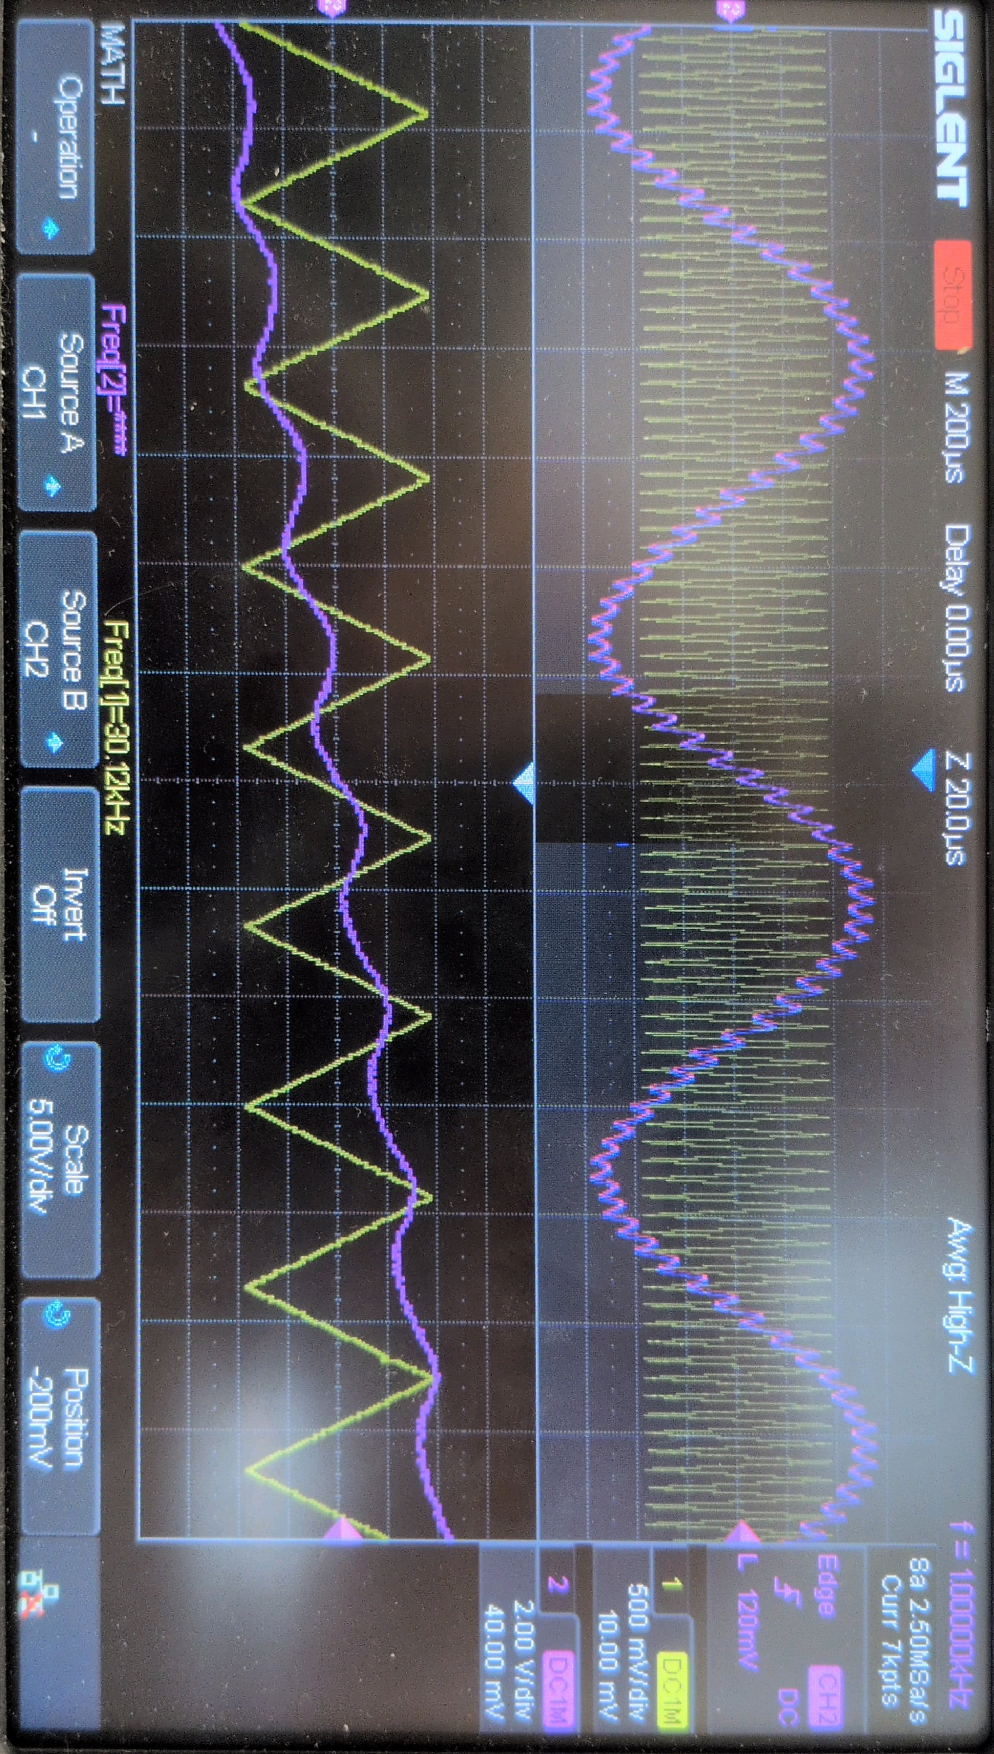
\includegraphics[height=\textwidth, angle=90]{osciloskop/DOC_20260317_112816.pdf}
    \caption{Porovnání vstupního signálu s referenčním pilovitým průběhem.}
\end{figure}

\subsection{Porovnání vstupního signálu s PWM modulovaným signálem}

\begin{figure}[H]
    \centering
    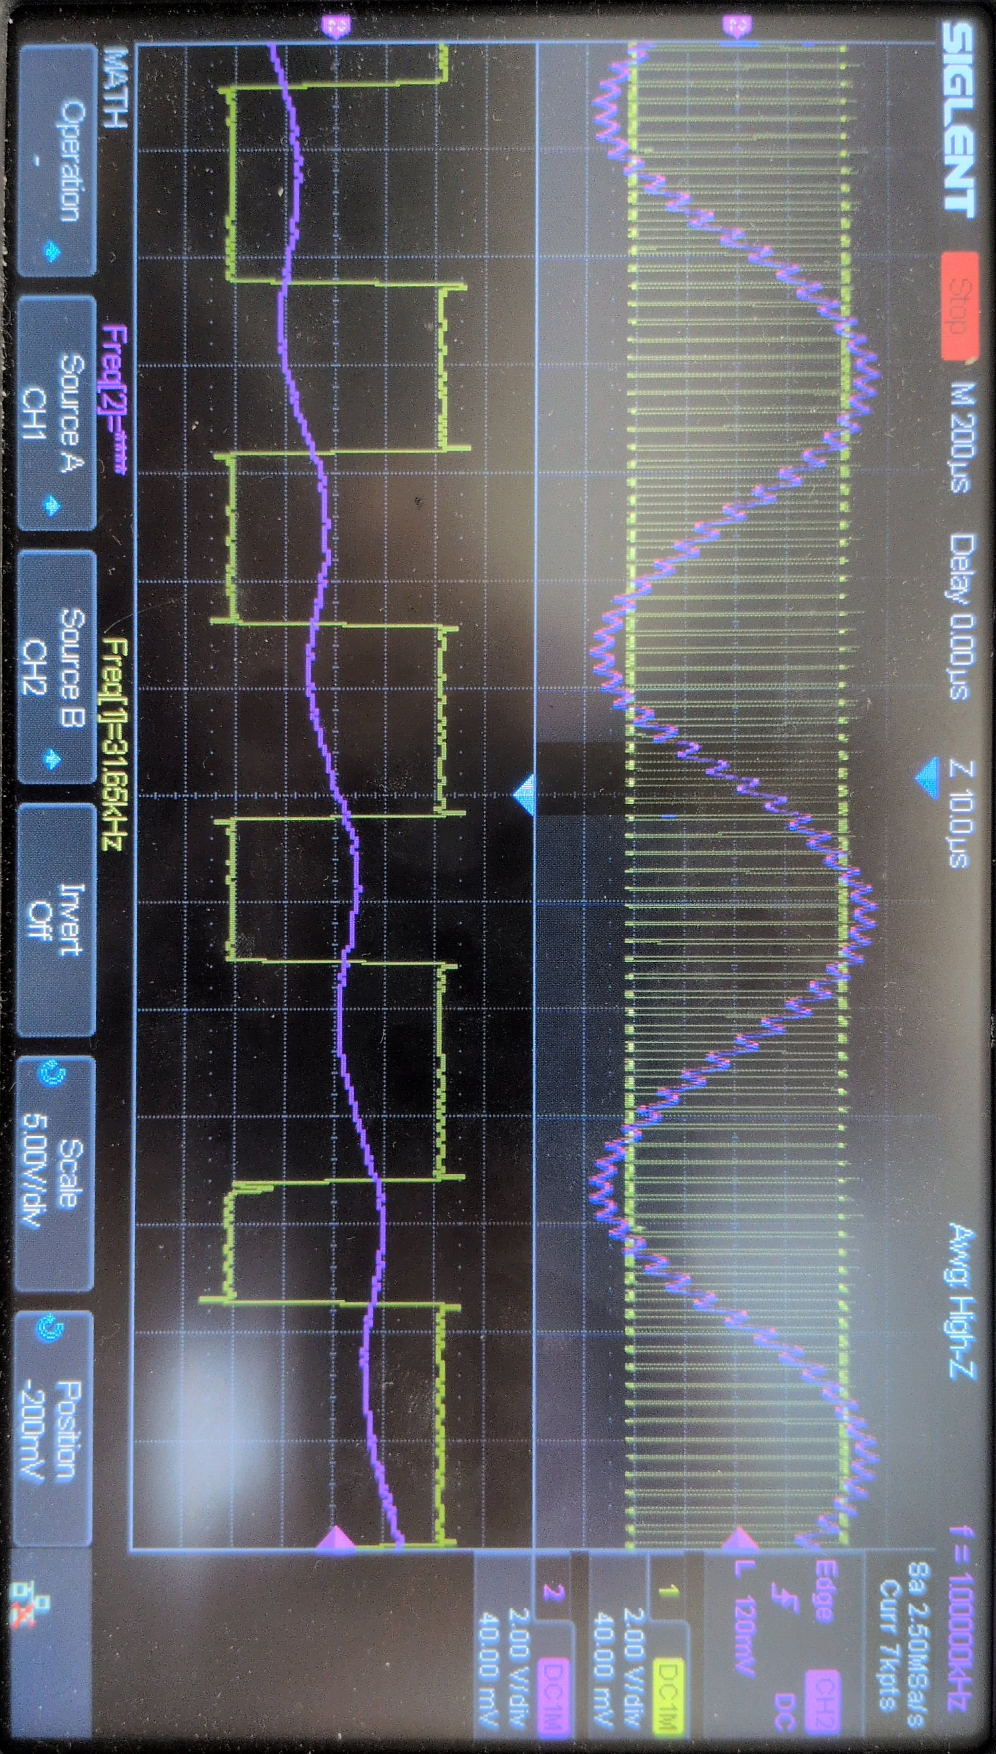
\includegraphics[height=\textwidth, angle=90]{osciloskop/DOC_20260317_113117.pdf}
    \caption{Porovnání vstupního signálu s PWM modulovaným signálem.}
\end{figure}

$t_\text{on} = 28\,\mu\text{s}$
$\ \ t_\text{off} = 32\,\mu\text{s}$
$\ \ s_\text{max} = \frac{28}{32} \cdot 100\,\% = 87{,}5\,\%$

$t_\text{on} = 5\,\mu\text{s}$
$\ \ t_\text{off} = 32\,\mu\text{s}$
$\ \ s_\text{min} = \frac{5}{32} \cdot 100\,\% = 15{,}625\,\%$

\subsection{Porovnání referenčního pilovitého signálu s PWM modulovaným signálem}

\begin{figure}[H]
    \centering
    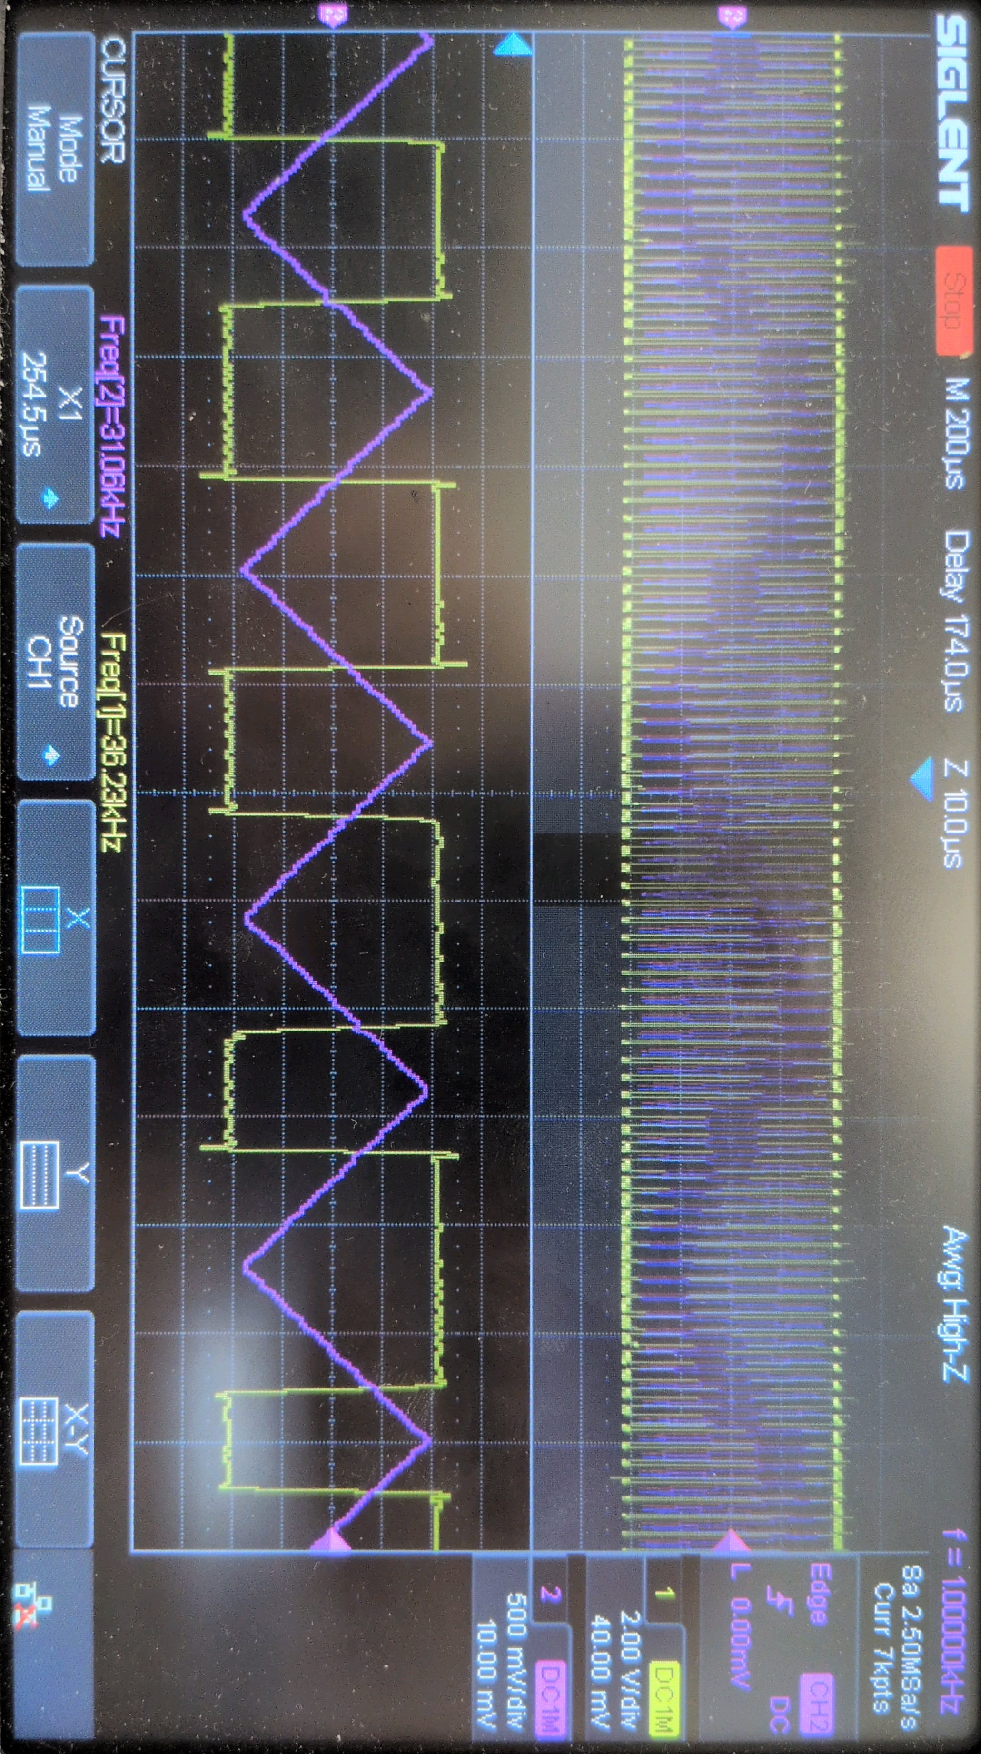
\includegraphics[height=\textwidth, angle=90]{osciloskop/DOC_20260317_114320.pdf}
    \caption{Porovnání referenčního pilovitého signálu s PWM modulovaným signálem.}
\end{figure}

\subsection{Porovnání průběhů na výstupu tranzistorového budiče budícího tranzistory T1 a T2}

\begin{figure}[H]
    \centering
    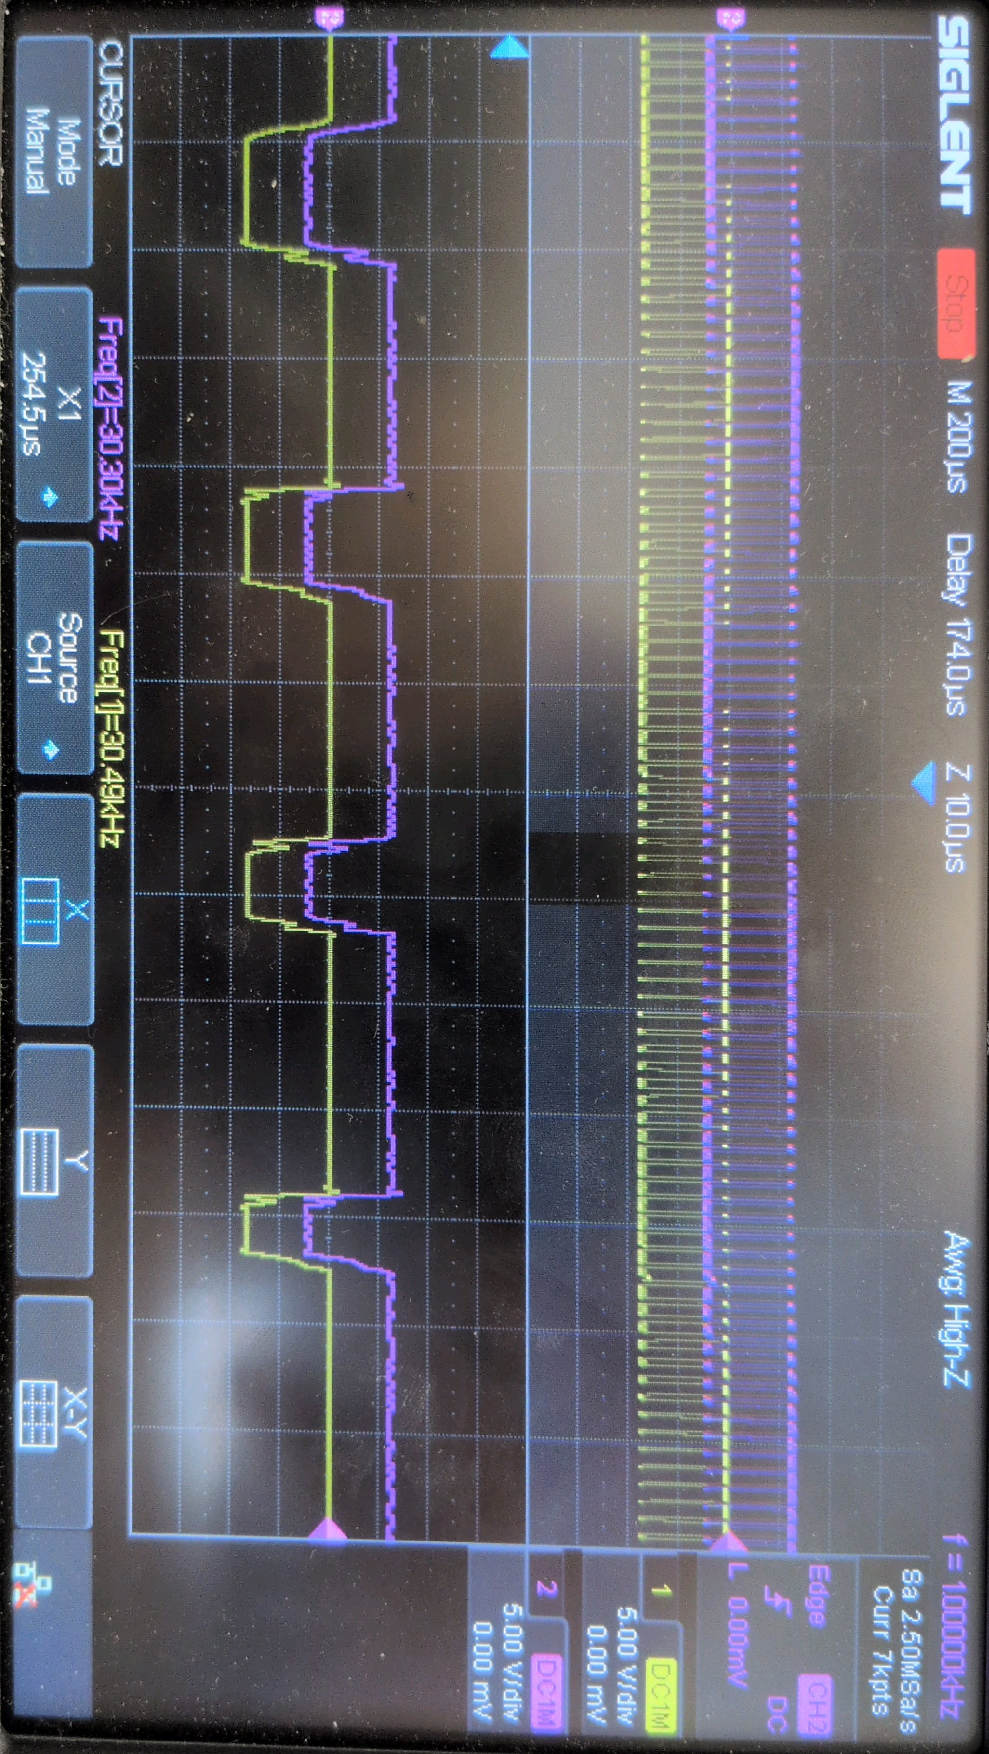
\includegraphics[height=\textwidth, angle=90]{osciloskop/DOC_20260317_114758.pdf}
    \caption{Porovnání průběhů na výstupu tranzistorového budiče budícího tranzistory T1 a T2.}
\end{figure}


\subsection{Porovnání průběhů za tranzistory T1, T2 a T3, T4}

\begin{figure}[H]
    \centering
    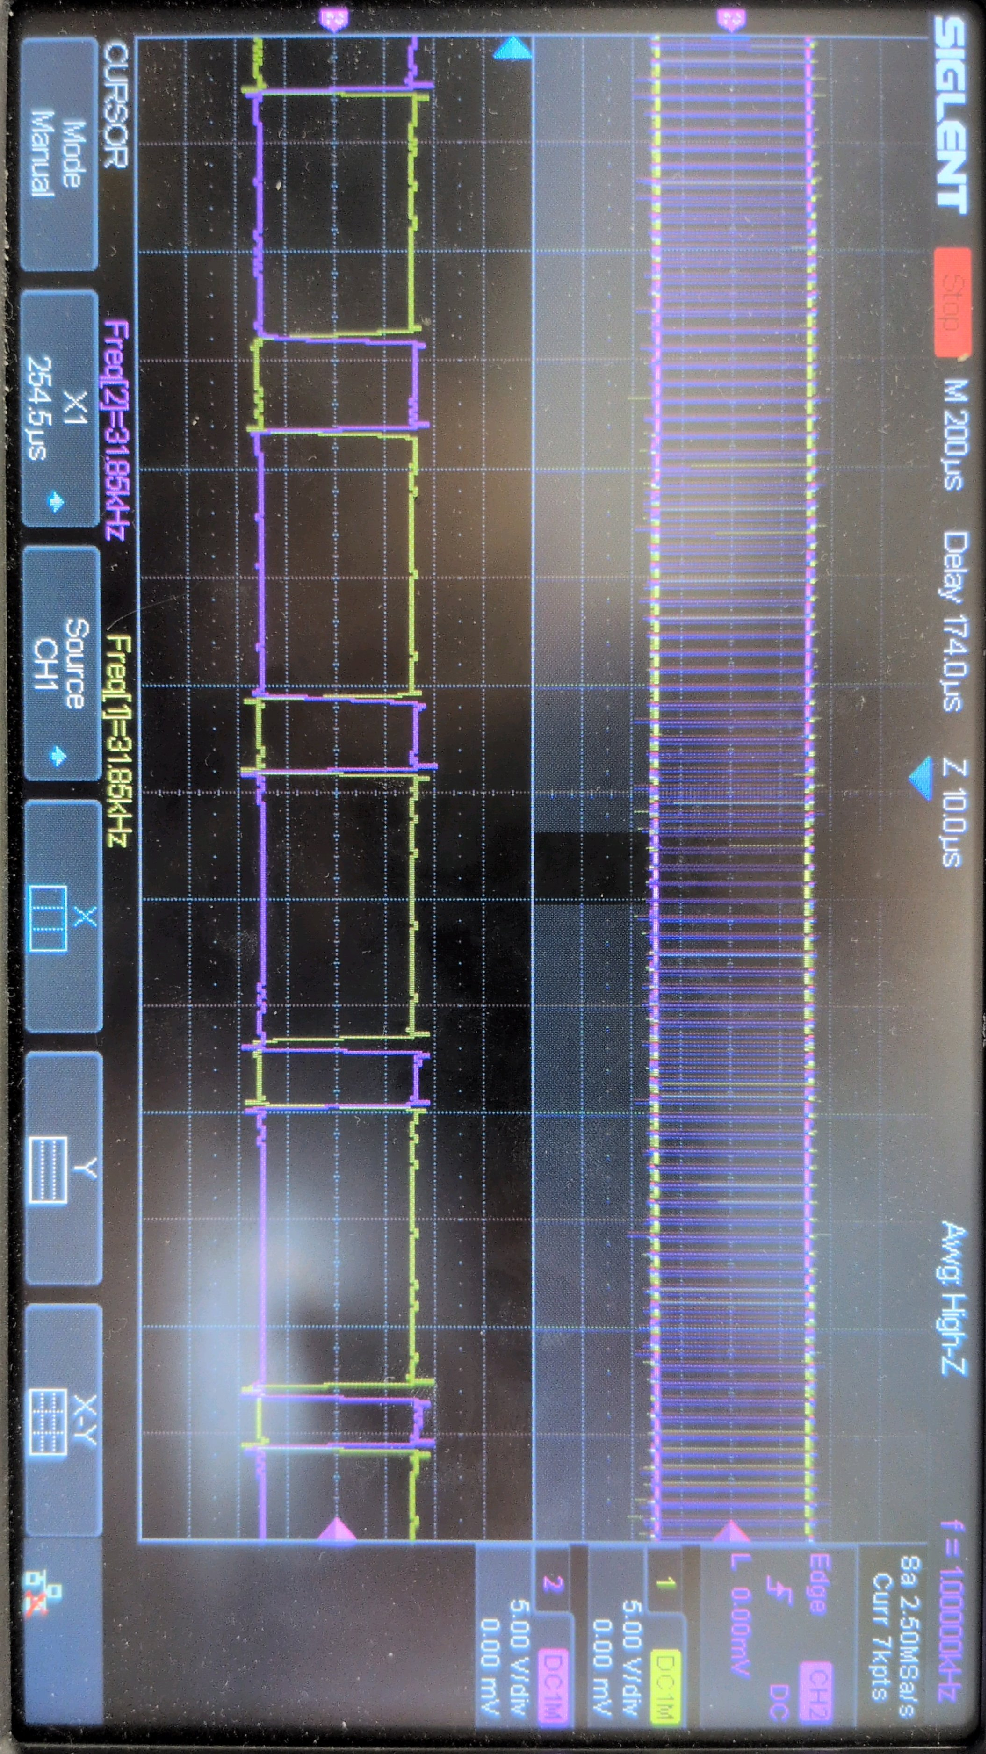
\includegraphics[height=\textwidth, angle=90]{osciloskop/DOC_20260317_114916.pdf}
    \caption{Porovnání průběhů za tranzistory T1, T2 a T3, T4.}
\end{figure}


\subsection{Porovnání výstupního zesíleného signálu modulu zesilovače se vstupním signálem}

\begin{figure}[H]
    \centering
    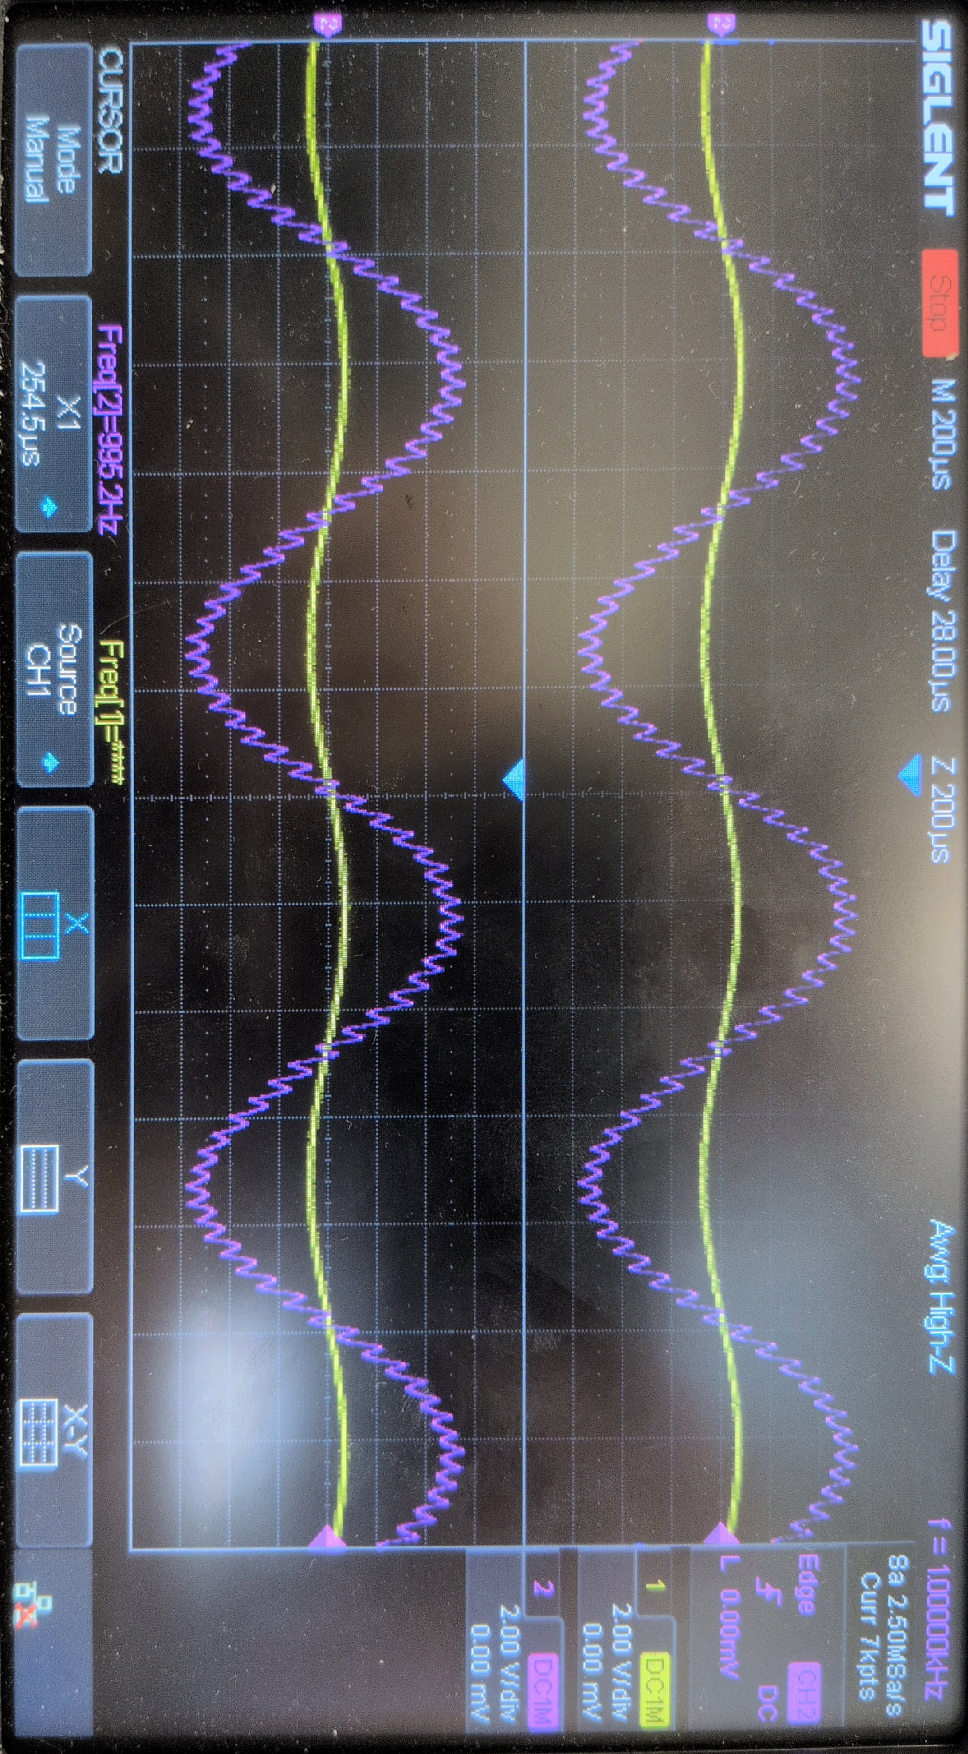
\includegraphics[height=\textwidth, angle=90]{osciloskop/DOC_20260317_115149.pdf}
    \caption{Porovnání výstupního zesíleného signálu modulu zesilovače se vstupním signálem.}
\end{figure}

\subsection{Můstkové zapojení}

\begin{figure}[H]
    \centering
    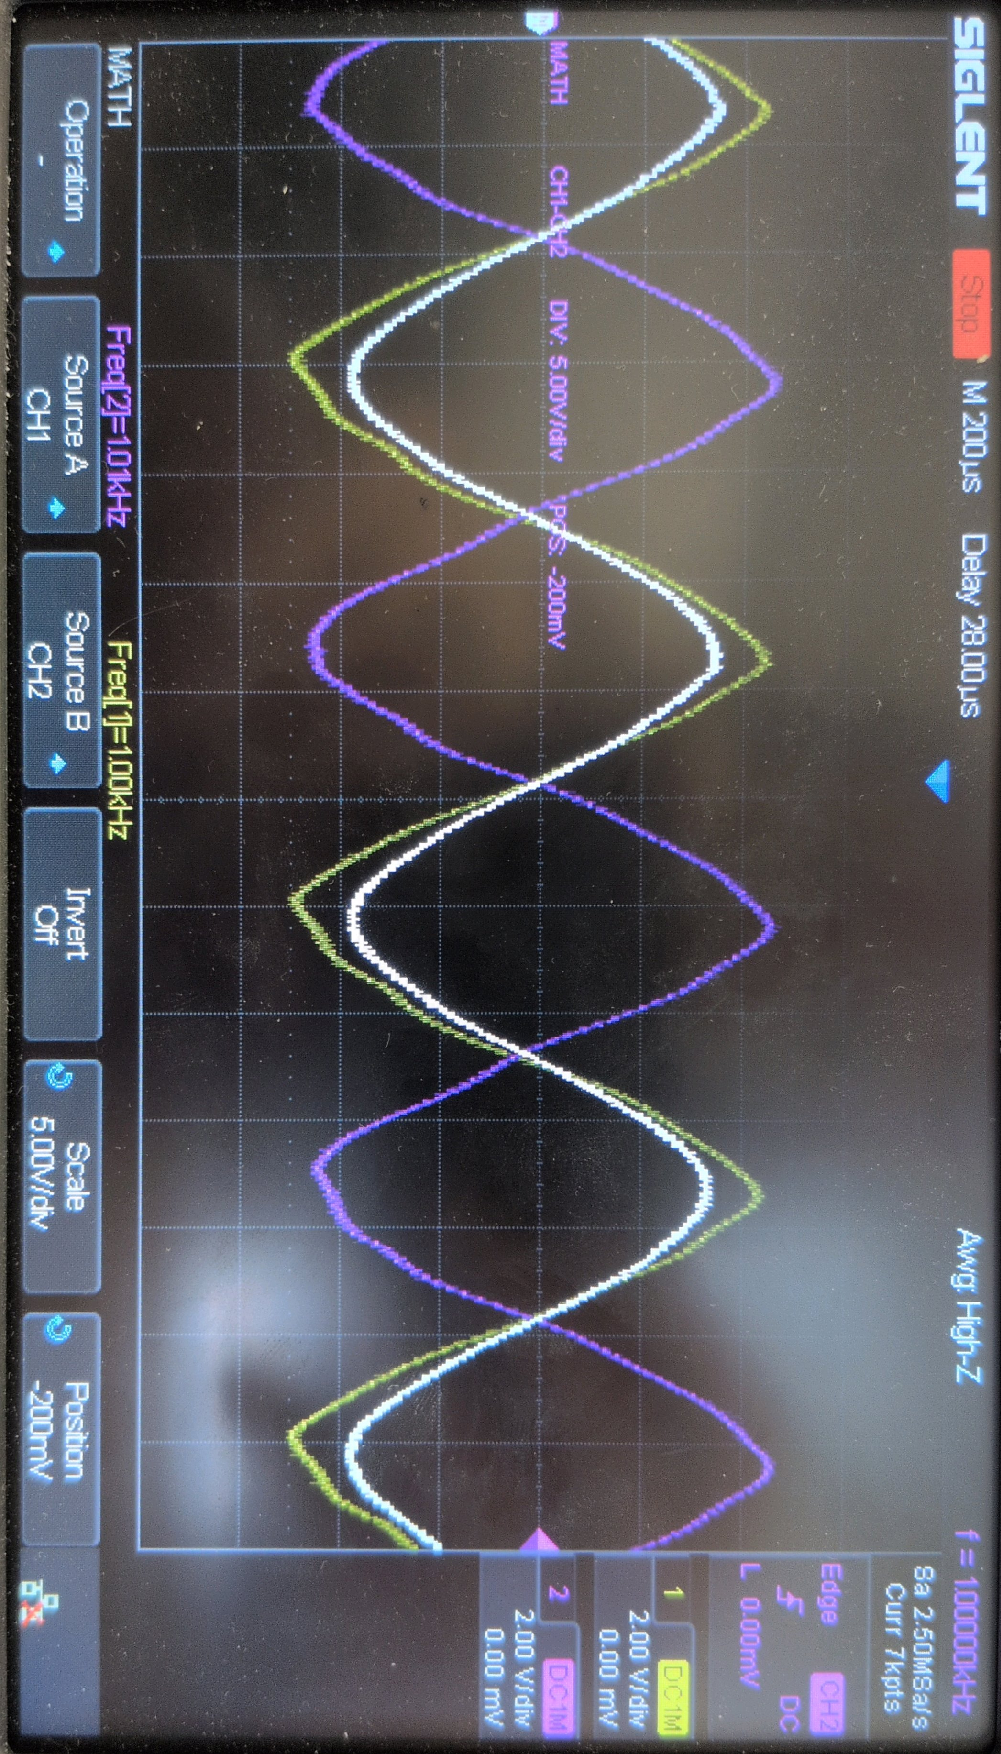
\includegraphics[height=\textwidth, angle=90]{osciloskop/DOC_20260317_120508.pdf}
    \caption{Můstkové zapojení.}
\end{figure}


\begin{itemize}
	\item \textbf{GEN} nízkofrekvenční funkční generátor Digimess FG100
	\item \textbf{OSC} paměťový osciloskop Agilent 54621A (60\,MHz)
	\item \textbf{NZ} napájecí zdroj Diametral P230R51D
	\item \textbf{LPT} tiskárna HP 5L připojená k osciloskopu
	\item měřený přípravek „Nízkofrekvenční zesilovač v třídě D“
	\item propojovací vodiče, 1 x BNC--BNC, 3 x osciloskopická sonda
\end{itemize}

\section{Závěr}

V prvním měření byla určena modulová kmitočtová charakteristika prvního kanálu zesilovače třídy D.
Nejvyšší zesílení bylo naměřeno při kmitočtu 3\,kHz, kde $A_\text{U\,dB} = 17{,}63\,\text{dB}$.
Při poklesu o 3\,dB vychází horní mezní kmitočet přibližně na 8\,kHz.
Dolní mezní kmitočet se nepodařilo v použitém rozsahu určit, protože ani při 50\,Hz nedošlo k poklesu o 3\,dB oproti maximu.
Z měření tedy plyne, že zesilovač v měřeném pásmu dobře pracuje přibližně do oblasti několika kilohertzů, poté jeho zesílení začne výrazněji klesat.

Z porovnání vstupního signálu s PWM modulovaným průběhem je patrné, že šířka impulzů závisí na okamžité hodnotě vstupního napětí.
Z naměřených časů byla stanovena maximální střída přibližně $87{,}5\,\%$ a minimální střída přibližně $15{,}63\,\%$, což potvrzuje správnou funkci PWM modulace.
Při porovnání s referenčním pilovitým signálem je zřejmé, že okamžik překlápění PWM signálu je určen průsečíkem vstupního a referenčního průběhu v komparátoru.

Na výstupech tranzistorového budiče a za tranzistory T1, T2 a T3, T4 byly pozorovány vzájemně opačné průběhy, což odpovídá komplementárnímu řízení výkonového stupně.
Na zesíleném výstupu modulu je již patrný užitečný nízkofrekvenční signál, ale současně i zbytkové zvlnění související se spínací frekvencí.
V můstkovém zapojení se amplituda výstupního napětí zvětšila díky rozdílu dvou opačných větví, a tím se zvýšil i dosažitelný výkon do zátěže.
Měření tak potvrdilo princip činnosti koncového zesilovače s PWM modulací i výhodu můstkového zapojení.

\end{document}